\section{Creating the Decision Support System}
\subsection{Chosing a problem}
The first step in solving the task for creating a decision support system is
selecting a problem for the system to solve. I have chosen to let the system
help in deciding the every-day-decision of what to do now, for a
regular student. For this kind of system, it is really hard to get real values
for the utility function, and also difficult to set default probabilities for
the environment. These values and probabilites must also be adjusted for each
subject, as different persons have different personalities, preferences and
work-effectiveness.


I have chosen the following activities that the system will help you decide
between:
\begin{itemize}
  \item Watch a movie with someone
  \item Watch a movie alone
  \item Do homework
  \item Eat dinner with someone
  \item Eat dinner alone
  \item Go to sleep
  \item Go outside
  \item Do excercise
\end{itemize}
of coure, there are a lot more things that could be added, but I think these are
a representative overall of actions.

\subsection{Decision parameters}
\index{parameters}Now that we have our problem defined, we need information
about the current state, in order to promote a good decision.

I have chosen some attributes that I think is important in order to decide what
to do, in the general context.

\begin{description}
\item[Lot to do] \hfill \\
Students have a \index{lot to do}lot to do, occasionally, but may also have a
lot of spare time.
Because how much you have to do is important deciding if you should do homework,
I have included this parameter.

\item[Hungry] \hfill \\
Whenever you are \index{hungry}hungry, it is a good idea to eat food.

\item[Sleepy] \hfill \\
You might be better off with sleeping than doing homework or doing excercises if
you are \index{sleepy}sleepy.

\item[Tired] \hfill \\
\index{tired}Tired is kind of a extended expression for sleepy, hungry, but also
general ``don't want to do nothing''. I have included this as a way of telling you are
tired, without beeing explicitly sleepy. If you are sleepy, of cource, this
affects tired, unless specified otherwise.

\item[Social needs] \hfill \\
Everyone has social needs from time to time, but sometimes, we also prefer
beeing alone. This is important deciding wherever we are going to spend time
alone, or meeting other people.

\item[Weather] \hfill \\
The \index{weather}weather is more an environmental condition, but is also
important for some decisions. We might say that it is more pleasing going out on a sunny
afternoon, then if it is a full storm outside. I would also state that there are
somewhat better to do homework while it is raining outside, since it lowers the
desire to go outside.

\end{description}

\subsection{The effect of a choise}
In order to calculate the \index{utility}utility value of a choise, we have to
look at its consequences. I have chosen some attributes that work as outcome of a choise and
a state. I have chosen to include the following consequence variables:
\begin{description}
\item[Usefullness] \hfill\\
I will argue that you feel better if you have done something usefull. Something
usefull depends on what demands you were having before doing an action, eg. if
you where hungry, it may be more usefull to eat something than to watch a movie,
and if you had a lot to do, it might be most usefull to do some homework.

\item[Work left] \hfill\\
How much work are we left with after doing our action. This is important because
it may be difficult to relax if you have much on your mind. Typically doing
homework leaves you with less to do, while sleeping leaves you with exactly the
same amout.

\item[Exhausting] \hfill\\
You might be more pleased with yourself if you have done something that was not
exhausting, since it leaves you with more energy. You might argue that it feels
good to be real exhausted after a hard excercise, but I have put those values
into \emph{Usefullness}, leaving just ``bad'' exhaustnes into this variable.

\item[Fun] \hfill\\
The more fun we have had, the better. Often, fun goes against usefullness, but
since some things might be fun and usefull, we need both variables.

\item[Social] \hfill\\
People have social demands, and this is important to how good we feel. If we
have little contact with other human beeings, we might feel lonely, while
over-stimulating the social life might not be too good either. 

\end{description}

\subsection{Compiling variables into a system}
The previous sections defined a set of variables and a set of choises that
makes up to a mini-world. The consepts of mini-worlds is that they models the
real world, or any world where we want to do computations. Of course, a more
advanced mini-world would be able to model the real world with better accuracy,
but would also (potensially) add severe complexity. In worst case, each variable
added would expand the model exponentially.

\begin{figure}[h]
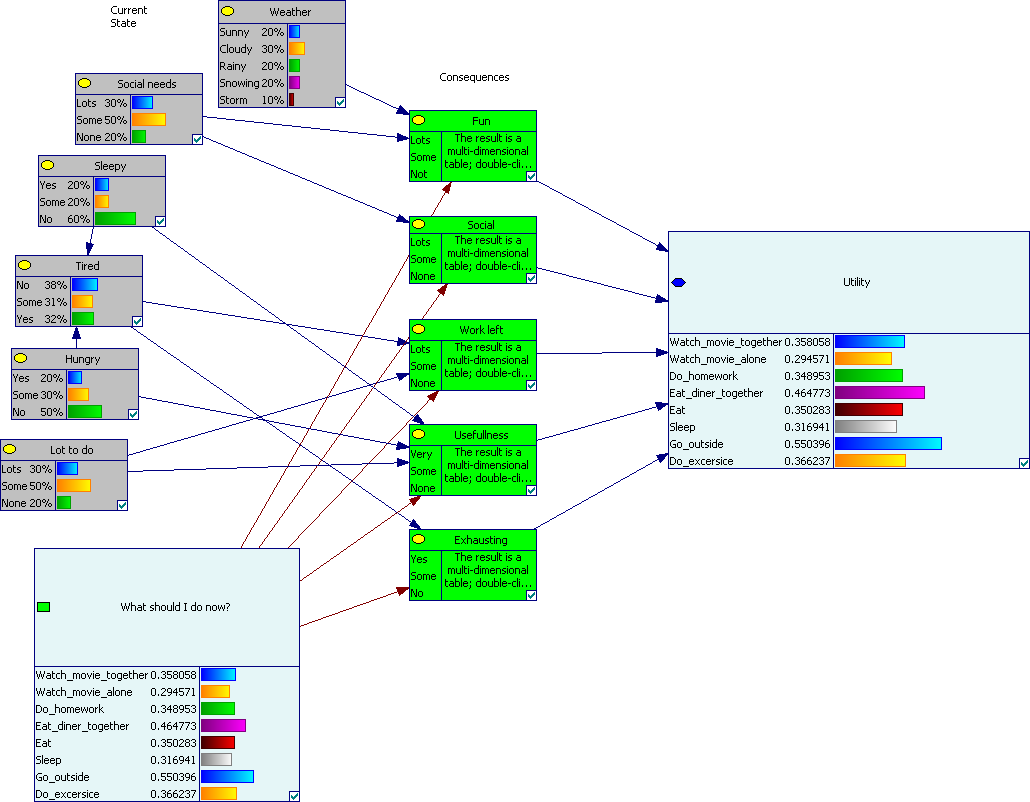
\includegraphics[width=154mm]{figure-complete.png}
\caption{Complete Decision Support System in GeNIe 2.0}
\end{figure}
